\section{Peripherals}
\label{sec:periphs}

The Basys2 has manny peripherals options such as:
-7-segments display
-on/off switch
-push buttons
-VGA port
-PS/2 port
-6-pin headers

\subsection{Peripherals Used}

The peripherals that we will de using are the 7-segments display and the push buttons.


\subsection{Timer Counter}

In the Timer we use this addresses.

\begin{table}[h]
\centering
\caption{Push Buttons.}
\sffamily
    \begin{tabular}{|c|c|c|c|c|c|c|}
        \hline
        \textbf{} & \textbf{Timer} & \textbf{min0} & \textbf{min1} & \textbf{hour0} & \textbf{hour1} \\ [0.5ex]
        \hline
        \hline
        BASE & 1600 & 1600 & 1601 & 1602 & 1603 \\
        \hline
        Addr\_W & 2 & - & - & - & - \\
        \hline
    \end{tabular}
\end{table}



\subsection{7-Segments Display}

The 7-segment displays will not need an memory address since it will receive the values to display directly from the timer module. For this to work we rely on the following diagram in the figure~\ref{fig:DisplayD}.

\begin{figure}[!h]
    \centerline{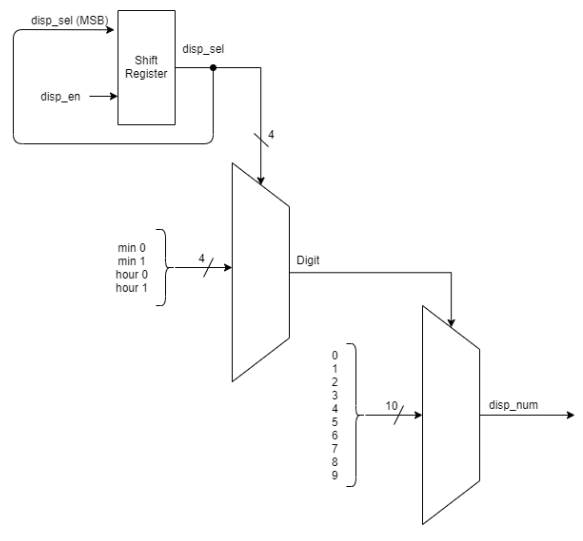
\includegraphics[width=15cm]{figures/83245571_235640547450606_3622537552461824000_n.png}}
    \vspace{0cm}\caption{Display Diagram}
    \label{fig:DisplayD}
\end{figure}



\subsection{Push Buttons}

\begin{table}[h]
\centering
\caption{Push Buttons.}
\sffamily
    \begin{tabular}{|c|c|c|c|}
        \hline
        \textbf{Name} & \textbf{Address} & \textbf{Bits} & \textbf{Description} \\ [0.5ex]
        \hline
        \hline
        BUTTON\_BASE & 1500 & 3:0 & Reset, mode, set hours and set minutes buttons\\
        \hline
    \end{tabular}
\end{table}

